\documentclass[11pt]{article}
\usepackage{scribe}
\usepackage{graphicx}

% Uncomment the appropriate line
%\Scribe{Your name}

\Scribes{Frendy Lio Can}
\LectureDate{November 12, 2020}
\LectureTitle{Homework Assignment \#6}

%\usepackage[mathcal]{euscript}


\begin{document}

\MakeScribeTop

%\paragraph{This is a paragraph heading} Paragraph.

%%%%%%%%%%%%%%%%%%%%%%%%%%%%%%%%
% PROBLEM 1 A
%%%%%%%%%%%%%%%%%%%%%%%%%%%%%%%%
\paragraph{\noindent\textbf{\LARGE{Problem 1, a)}}}

\begin{equation*}
\begin{split}
    E[||x-x^*||^2]  = & E[(x -y^T\theta)^2] \\
                    = & E[x^2 - 2\theta^Tyx + \theta^T y y^T \theta] \\
                    = & E[x^2] -2\theta^T E[yx] + \theta^T E[y y^t] \theta \\
                    = & \sigma^2 - 2\theta^Tr_{y,x} + \theta^TC_y\theta
\end{split}
\end{equation*}


%%%%%%%%%%%%%%%%%%%%%%%%%%%%%%%%
% PROBLEM 1 B
%%%%%%%%%%%%%%%%%%%%%%%%%%%%%%%%
\paragraph{\noindent\textbf{\LARGE{Problem 1, b)}}}

\begin{equation*}
\begin{split}
    \operatorname*{argmin}_\theta E[||x-x^*||^2]  = & \frac{\partial}{\partial \theta}  E[||x-x^*||^2]\\
        = & \frac{\partial}{\partial \theta}  [\sigma^2 - 2\theta^Tr_{y,x} + \theta^TC_y\theta] \\
        = & - 2r_{y,x} + 2C_y\theta \\
        = & 0 \\
        \text{Therefore} & \\
    \theta = & C_y^{-1} r_{y,x} 
\end{split}
\end{equation*}

        
%%%%%%%%%%%%%%%%%%%%%%%%%%%%%%%%
% PROBLEM 1 C
%%%%%%%%%%%%%%%%%%%%%%%%%%%%%%%%
\paragraph{\noindent\textbf{\LARGE{Problem 1, c)}}}  
\begin{equation*}
\begin{split}
    C_y = & E[yy^T] \\
        = & E[(ax+n)(ax+n)^T] \\
        = & E[x^2aa^T + xan^T + xna^T + nn^T] \\
        = & E[x^2]aa^T + E[xn^T]a + E[xn]a^T + E[nn^T] \\
    \text{Since } &  n \text{ is independent}. E[xn] = E[xn^T] = 0\\
        = & \sigma^2 aa^T + 0 + 0 + C_n \\
        = & \sigma^2 aa^T  + C_n \\
\end{split}
\end{equation*}

%%%%%%%%%%%%%%%%%%%%%%%%%%%%%%%%
% PROBLEM 1 D
%%%%%%%%%%%%%%%%%%%%%%%%%%%%%%%%
\paragraph{\noindent\textbf{\LARGE{Problem 1, d)}}}  
\begin{equation*}
\begin{split}
    r_{y,x} = & E[yx] \\
        = & E[(ax+n)(x)] \\
        = & E[ax^2 + nx] \\
        = & aE[x^2] + E[n]E[x] \\
        = & \sigma^2 a + 0 \\
        = & \sigma^2 a 
\end{split}
\end{equation*}

%%%%%%%%%%%%%%%%%%%%%%%%%%%%%%%%
% PROBLEM 1 E
%%%%%%%%%%%%%%%%%%%%%%%%%%%%%%%%
\paragraph{\noindent\textbf{\LARGE{Problem 1, e)}}}  
\begin{equation*}
\begin{split}
    x^* = & y^T\theta \\
        = & y^T C_y^{-1} r_{y,x}  \\
        = & (ax + n)^T (\sigma^2 aa^T  + C_n)^{-1} \sigma^2 a 
\end{split}
\end{equation*}


%%%%%%%%%%%%%%%%%%%%%%%%%%%%%%%%
% PROBLEM 2 a
%%%%%%%%%%%%%%%%%%%%%%%%%%%%%%%%
\paragraph{\noindent\textbf{\LARGE{Problem 2, a)}}}  
  
\begin{equation*}
\begin{split}
    E[MSE_{2} (\hat{\theta})]  = & E[\frac{1}{M} \sum_{n \in S_2 }||x_n - f(y_n, \hat{\theta} )||^2_2] \\
            = &  \frac{1}{M} E[ \sum_{n \in S_2 }||x_n - f(y_n, \hat{\theta} )||^2_2] \\
            = &  \frac{1}{M} \sum_{n \in S_2 } E[ ||x_n - f(y_n, \hat{\theta} )||^2_2] \\
\end{split}
\end{equation*}
\begin{flushleft}
    Since when we know that $\hat{\theta} > \theta^*$.
\end{flushleft}  
\begin{equation*}
\begin{split}
    \frac{1}{M} \sum_{n \in S_2 } E[ ||x_n - f(y_n, \hat{\theta} )||^2_2] \geq & \frac{1}{M} \sum_{n \in S_2 } E[ ||x_n - f(y_n,\theta^* )||^2_2] \\
    E[MSE_2(\hat{\theta})] \geq & E[MSE_2 \theta^*]
\end{split}
\end{equation*}
\begin{flushleft}
    Thus, $MSE_2(\theta^*)$ is smaller.
\end{flushleft}  

%%%%%%%%%%%%%%%%%%%%%%%%%%%%%%%%
% PROBLEM 2 b
%%%%%%%%%%%%%%%%%%%%%%%%%%%%%%%%
\paragraph{\noindent\textbf{\LARGE{Problem 2, b)}}}  
  
\begin{flushleft}
    We will need to know the distribution of $x_n$ and $y_n$. This values are usually not given/available.
\end{flushleft}  

%%%%%%%%%%%%%%%%%%%%%%%%%%%%%%%%
% PROBLEM 2 c
%%%%%%%%%%%%%%%%%%%%%%%%%%%%%%%%
\paragraph{\noindent\textbf{\LARGE{Problem 2, c)}}}  
  
\begin{flushleft}
    I think L needs to be at least larger than $p$, where $p$ is the dimension of $\theta (\theta \in R^p)$. Is also important to note that if $L \Rightarrow \infty$, the better $\hat{\theta}$ becomes.
\end{flushleft} 
 
%%%%%%%%%%%%%%%%%%%%%%%%%%%%%%%%
% PROBLEM 2 d
%%%%%%%%%%%%%%%%%%%%%%%%%%%%%%%%
\newpage
\paragraph{\noindent\textbf{\LARGE{Problem 2, d)}}}  

\begin{flushleft}
    \begin{figure}[htbp]
        \centerline{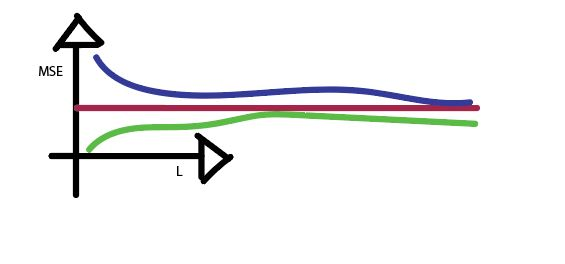
\includegraphics[scale=.5]{graph.JPG}}
        \caption{Problem 2-d}
        \label{fig}
    \end{figure}

    Blue Line (Top line) is $MSE_2\hat{\theta}$ \\
    Purple Line (Middle Line) is $MSE_2(\theta^*)$ \\
    Green Line (Bottom Line) is $MSE_1(\hat{\theta})$
\end{flushleft}

%%%%%%%%%%%%%%%%%%%%%%%%%%%%%%%%
% PROBLEM 3 e
%%%%%%%%%%%%%%%%%%%%%%%%%%%%%%%%
\paragraph{\noindent\textbf{\LARGE{Problem 3, e)}}}  
  
\begin{flushleft}
    The PSNR for the moving average filter $(22.8478)$ is worst than the learned filter $(24.9928)$.
\end{flushleft} 
 
\end{document}
